\chapter{The EPR ``theorem''}

In this chapter...

\section{Perfect correlations in systems of two spin-1/2 particles}

\begin{figure}
  \centering
  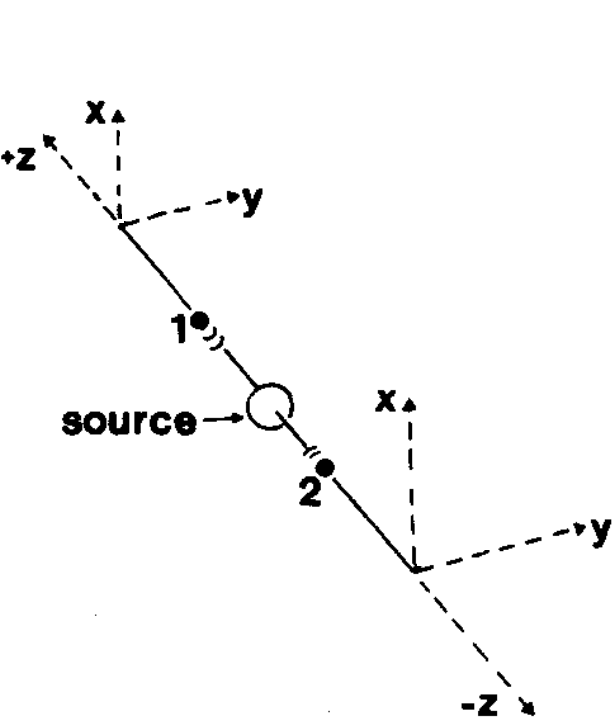
\includegraphics[width=0.275\textwidth]{Mainmatter/Chapter1/eprb-gedankenexperiment.png}
  \caption{}
  \label{fig:eprb-gedankenexperiment}
\end{figure}

In this section we will present some aspects of the quantum mechanical description of systems composed of two spin-1/2 particles. In particular we will show that there exist situations for which quantum mechanics predicts perfect correlations between the results of measurements performed on the two particles. We will also see that such correlations are independent of where and when the two measurements are performed.%is it clear enough that the two measurements are made on the two particles separately?

Consider for instance two spin-1/2 particles emited at a source and propagating in opposite directions along the $\mathbf{\hat{z}}$ axis (see Fig. \ref{fig:eprb-gedankenexperiment}).  Each particle then enters an apparatus (e.g. a Stern-Gerlach magnet) that can measure either the $S_x$ or $S_y$ spin component. Suppose that the two particles are emited in the state with total spin equal to $0$, that is:
\begin{equation}
  |\chi\rangle = \frac{1}{\sqrt{2}} \left( |+\rangle_1 |-\rangle_2 - |-\rangle_1 |+\rangle_2 \right)
  \label{eq:singlet-state}
\end{equation}
where the vectors $|+\rangle_i$ and $|-\rangle_i$ represent, respectively, states of spin up and down along an arbitrary direction $\mathbf{\hat{n}}$ for particle $i = 1, 2$. The state (\ref{eq:singlet-state}) is such as to take the same form indipendently of $\mathbf{\hat{n}}$, thus no ambiguity arises from omitting the direction $\mathbf{\hat{n}}$ in the notation (see Appendix \ref{app:spin-rotations} for a proof of this statement). This last statement also allows us to easily see that if the two measuring apparatuses happen to be oriented in the same direction, that is if they both measure either the $S_x$ or $S_y$ spin component, then the spins of the two particles will be found to have opposite sign.

\begin{observation}
  Notice that the perfect correlations we have predicted in this section are independent on the time order with which we perform the two measurements as well as on the distance between the places where the two measuring apparatuses are located.%should I add something like: ``as long as the spin state doesn't change''?
\end{observation}

\begin{observation}
  The appearence of correlations between the results of the two spin measurements considered are ENTANGLEMENT.
\end{observation}

\begin{observation}
  In this section we made use of labels for the two particles.
SPATIAL PART OF THE WAVEFUNCTION
\end{observation}


\section{EPR argument}
In this section we will present the argument proposed by Einstein, Podolsky and Rosen \cite{PhysRev.47.777} to prove that quantum mechanics is incomplete.

\begin{note}
Throughout the presentation of the argument we will refer to the experimental conditions considered in the previous section.
\end{note}

Let us start by stating clearly all the assumtions on which the argument rests. The first of these is the prediction of quantum mechanics we have derived in the previuos section, that is:
\begin{enumerate}
  %enumerated lists style
  \renewcommand{\theenumi}{\alph{enumi}}
  \renewcommand{\labelenumi}{(\theenumi)}
\item \label{itm:epr-perfect-correlations} \textit{Perfect correlation:} If the spins of the two particles are measured along the same direction, then the two spins will be found (with certainity) to have opposite sign (independently of the time order and spatial distance at which the two measurements are performed).
\end{enumerate}
We then assume the validity of the following (necessary) requirement for a theory to be complete:
\begin{enumerate}
  \setcounter{enumi}{1}
  %enumerated lists style
  \renewcommand{\theenumi}{\alph{enumi}}
  \renewcommand{\labelenumi}{(\theenumi)}
\item \label{itm:epr-completeness} \textit{Completeness:} ``Every element of the physical reality must have a counterpart in the [complete] physical theory.'' \cite{PhysRev.47.777}
\end{enumerate}
Where to identify the \textit{elements of the physical reality} we assume the validity of the (sufficient) criterion that follows:
\begin{enumerate}
  \setcounter{enumi}{2}
  %enumerated lists style
  \renewcommand{\theenumi}{\alph{enumi}}
  \renewcommand{\labelenumi}{(\theenumi)}
\item \label{itm:epr-reality} \textit{Reality:} ``If, without in any way disturbing a system, we can predict with certainity (i.e. with probability equal to unity) the value of a physical quantity, then there exist an element of physical reality corresponding to this physical quantity.'' \cite{PhysRev.47.777}
\end{enumerate}
At last we assume that the two measuring apparatuses are very far form each other, thus, again in EPR words \cite{PhysRev.47.777}:
\begin{enumerate}
  \setcounter{enumi}{3}
  %enumerated lists style
  \renewcommand{\theenumi}{\alph{enumi}}
  \renewcommand{\labelenumi}{(\theenumi)}
\item \label{itm:epr-locality} \textit{Locality:} ``Since at the time of measurement the two systems [the two particles in our case] no longer interact, no real change [\footnote{By ``real change'' we mean changes to the \textit{elements of the physical reality}}] can take place in the second system in consequence of anything that may be done to the first system.''
\end{enumerate}

The argument is then the following: Suppose a spin component, say $S_x$ ($S_y$), of particle 1 is measured at some time $t_1$, because of the perfect correlation assumption (\ref{itm:epr-perfect-correlations}), we know that if at some time $t_2 > t_1$ the same spin component of particle 2 is measured it will be found (with certainity) to have opposite sign. Locality, (\ref{itm:epr-locality}), ensures that the elements of physical reality associated to particle 2 have not changed as a consequnce of the measurement performed on particle 1. Thus, by the reality assumption (\ref{itm:epr-reality}), there is an element of physical reality corresponding to the $S_x$ ($S_y$) physical quantity of particle 2. Using again (\ref{itm:epr-locality}) we can state that such element of physical reality existed before the measurement on particle 1 was performed. Exchanging the role of the two particles in the previous steps leads to the conclusion that there corresponds an element of physical reality also to the $S_x$ ($S_y$) physical quantity of particle 1, this element of physical reality too existed before \textit{any} measurement was performed. We have thus obtained that the results of the two measurements were predetermined. Since the quantum state considered, (\ref{eq:singlet-state}), does not determine the result of the two measurements, we conclude that the theory ignores the elements of reality whe have found to exist and, by completeness (\ref{itm:epr-completeness}), must be considered incomplete. This completes the proof of the EPR ``theorem''.%is the final step clear enough or is it better to go Laloe's way? - is the S_y thing clear enough? - is it clear that the state considered at the beginning is the singlet one?

\begin{observation}
  ORIGINAL EPR: NO INTERACTION VS LOCALITY - FINAL PART OF THE ARGUMENT DIFFERS
\end{observation}

\begin{observation}
  ELEMENTS OF PHYSICAL REALITY CANNOT BE IN MEASURING APPARATUS \cite{}
\end{observation}

\begin{observation}
  ASSOCIATED VS SPACE REGION - SEPARABILITY
\end{observation}

\begin{observation}
  DEPENDENCE ON MEASURING APPARATUS SETTINGS
\end{observation}
